%!TEX TS-program = xelatex
\documentclass[10pt,oneside]{article}
\usepackage[fontsize=9pt]{scrextend}

\usepackage[english]{babel}

\usepackage{amsmath,amssymb,amsfonts}
\usepackage[utf8]{inputenc}
\usepackage[T1]{fontenc}
\usepackage{stix2}
\usepackage[scaled]{helvet}
\usepackage[scaled]{inconsolata}

\usepackage{lastpage}

\usepackage{setspace}

\usepackage{ccicons}

\usepackage[hang,flushmargin]{footmisc}

\usepackage{geometry}

\setlength{\parindent}{0pt}
\setlength{\parskip}{6pt plus 2pt minus 1pt}

\usepackage{fancyhdr}
\renewcommand{\headrulewidth}{0pt}\providecommand{\tightlist}{%
  \setlength{\itemsep}{0pt}\setlength{\parskip}{0pt}}

\makeatletter
\newcounter{tableno}
\newenvironment{tablenos:no-prefix-table-caption}{
  \caption@ifcompatibility{}{
    \let\oldthetable\thetable
    \let\oldtheHtable\theHtable
    \renewcommand{\thetable}{tableno:\thetableno}
    \renewcommand{\theHtable}{tableno:\thetableno}
    \stepcounter{tableno}
    \captionsetup{labelformat=empty}
  }
}{
  \caption@ifcompatibility{}{
    \captionsetup{labelformat=default}
    \let\thetable\oldthetable
    \let\theHtable\oldtheHtable
    \addtocounter{table}{-1}
  }
}
\makeatother

\usepackage{array}
\newcommand{\PreserveBackslash}[1]{\let\temp=\\#1\let\\=\temp}
\let\PBS=\PreserveBackslash

\usepackage[breaklinks=true]{hyperref}
\hypersetup{colorlinks,%
citecolor=blue,%
filecolor=blue,%
linkcolor=blue,%
urlcolor=blue}
\usepackage{url}

\usepackage{caption}
\setcounter{secnumdepth}{0}
\usepackage{cleveref}

\usepackage{graphicx}
\makeatletter
\def\maxwidth{\ifdim\Gin@nat@width>\linewidth\linewidth
\else\Gin@nat@width\fi}
\makeatother
\let\Oldincludegraphics\includegraphics
\renewcommand{\includegraphics}[1]{\Oldincludegraphics[width=\maxwidth]{#1}}

\usepackage{longtable}
\usepackage{booktabs}

\usepackage{color}
\usepackage{fancyvrb}
\newcommand{\VerbBar}{|}
\newcommand{\VERB}{\Verb[commandchars=\\\{\}]}
\DefineVerbatimEnvironment{Highlighting}{Verbatim}{commandchars=\\\{\}}
% Add ',fontsize=\small' for more characters per line
\usepackage{framed}
\definecolor{shadecolor}{RGB}{248,248,248}
\newenvironment{Shaded}{\begin{snugshade}}{\end{snugshade}}
\newcommand{\KeywordTok}[1]{\textcolor[rgb]{0.13,0.29,0.53}{\textbf{#1}}}
\newcommand{\DataTypeTok}[1]{\textcolor[rgb]{0.13,0.29,0.53}{#1}}
\newcommand{\DecValTok}[1]{\textcolor[rgb]{0.00,0.00,0.81}{#1}}
\newcommand{\BaseNTok}[1]{\textcolor[rgb]{0.00,0.00,0.81}{#1}}
\newcommand{\FloatTok}[1]{\textcolor[rgb]{0.00,0.00,0.81}{#1}}
\newcommand{\ConstantTok}[1]{\textcolor[rgb]{0.00,0.00,0.00}{#1}}
\newcommand{\CharTok}[1]{\textcolor[rgb]{0.31,0.60,0.02}{#1}}
\newcommand{\SpecialCharTok}[1]{\textcolor[rgb]{0.00,0.00,0.00}{#1}}
\newcommand{\StringTok}[1]{\textcolor[rgb]{0.31,0.60,0.02}{#1}}
\newcommand{\VerbatimStringTok}[1]{\textcolor[rgb]{0.31,0.60,0.02}{#1}}
\newcommand{\SpecialStringTok}[1]{\textcolor[rgb]{0.31,0.60,0.02}{#1}}
\newcommand{\ImportTok}[1]{#1}
\newcommand{\CommentTok}[1]{\textcolor[rgb]{0.56,0.35,0.01}{\textit{#1}}}
\newcommand{\DocumentationTok}[1]{\textcolor[rgb]{0.56,0.35,0.01}{\textbf{\textit{#1}}}}
\newcommand{\AnnotationTok}[1]{\textcolor[rgb]{0.56,0.35,0.01}{\textbf{\textit{#1}}}}
\newcommand{\CommentVarTok}[1]{\textcolor[rgb]{0.56,0.35,0.01}{\textbf{\textit{#1}}}}
\newcommand{\OtherTok}[1]{\textcolor[rgb]{0.56,0.35,0.01}{#1}}
\newcommand{\FunctionTok}[1]{\textcolor[rgb]{0.00,0.00,0.00}{#1}}
\newcommand{\VariableTok}[1]{\textcolor[rgb]{0.00,0.00,0.00}{#1}}
\newcommand{\ControlFlowTok}[1]{\textcolor[rgb]{0.13,0.29,0.53}{\textbf{#1}}}
\newcommand{\OperatorTok}[1]{\textcolor[rgb]{0.81,0.36,0.00}{\textbf{#1}}}
\newcommand{\BuiltInTok}[1]{#1}
\newcommand{\ExtensionTok}[1]{#1}
\newcommand{\PreprocessorTok}[1]{\textcolor[rgb]{0.56,0.35,0.01}{\textit{#1}}}
\newcommand{\AttributeTok}[1]{\textcolor[rgb]{0.77,0.63,0.00}{#1}}
\newcommand{\RegionMarkerTok}[1]{#1}
\newcommand{\InformationTok}[1]{\textcolor[rgb]{0.56,0.35,0.01}{\textbf{\textit{#1}}}}
\newcommand{\WarningTok}[1]{\textcolor[rgb]{0.56,0.35,0.01}{\textbf{\textit{#1}}}}
\newcommand{\AlertTok}[1]{\textcolor[rgb]{0.94,0.16,0.16}{#1}}
\newcommand{\ErrorTok}[1]{\textcolor[rgb]{0.64,0.00,0.00}{\textbf{#1}}}
\newcommand{\NormalTok}[1]{#1}

\newlength{\cslhangindent}
\setlength{\cslhangindent}{1.5em}
\newlength{\csllabelwidth}
\setlength{\csllabelwidth}{3em}
\newenvironment{CSLReferences}[3] % #1 hanging-ident, #2 entry spacing
 {% don't indent paragraphs
  \setlength{\parindent}{0pt}
  % turn on hanging indent if param 1 is 1
  \ifodd #1 \everypar{\setlength{\hangindent}{\cslhangindent}}\ignorespaces\fi
  % set entry spacing
  \ifnum #2 > 0
  \setlength{\parskip}{#2\baselineskip}
  \fi
 }%
 {}
\usepackage{calc} % for \widthof, \maxof
\newcommand{\CSLBlock}[1]{#1\hfill\break}
\newcommand{\CSLLeftMargin}[1]{\parbox[t]{\maxof{\widthof{#1}}{\csllabelwidth}}{#1}}
\newcommand{\CSLRightInline}[1]{\parbox[t]{\linewidth}{#1}}
\newcommand{\CSLIndent}[1]{\hspace{\cslhangindent}#1}\usepackage[table,dvipsnames]{xcolor}

\geometry{includemp,
            letterpaper,
            top=2.4cm,
            bottom=2.4cm,
            left=1.0cm,
            right=1.0cm,
            marginparwidth=5cm,
            marginparsep=1.0cm}

\usepackage[singlelinecheck=off]{caption}

\captionsetup{
  font={small},
  labelfont={bf},
  format=plain,
  labelsep=quad
}

\usepackage{floatrow}

\floatsetup[figure]{margins=hangright,
              facing=no,
              capposition=beside,
              capbesideposition={center,outside},
              floatwidth=\textwidth}

% \floatsetup[table]{margins=hangright,
%              facing=no,
%              capposition=beside,
%              capbesideposition={center,outside},
%              floatwidth=\textwidth}

\pagestyle{plain}

\setcounter{secnumdepth}{5}

\usepackage{titlesec}

\titleformat{\section}[block]
{\normalfont\large\sffamily}
{\thesection}{.5em}{\titlerule\\[.8ex]\bfseries}

\titleformat{\subsection}[runin]
{\normalfont\fontseries{b}\selectfont\filright\sffamily}
{\thesubsection.}{.5em}{}

\titleformat{\subsubsection}[runin]
{\normalfont\itshape\rmfamily\bfseries}{\thesubsubsection}{1em}{}

\fancypagestyle{firstpage}
{
   \fancyhf{}
   \renewcommand{\headrulewidth}{0pt}
   \fancyfoot[R]{\footnotesize\ccby}
   \fancyfoot[L]{\footnotesize\sffamily\today}
}

\fancypagestyle{normal}
{
  \fancyhf{}
  \fancyfoot[R]{\footnotesize\sffamily\thepage\ of \pageref*{LastPage}}
}

\usepackage{tikz}
\begin{document}
\pagestyle{normal}
\thispagestyle{firstpage}

\newcommand{\colorRule}[3][black]{\textcolor[HTML]{#1}{\rule{#2}{#3}}}

\noindent {\LARGE \textbf{\textsf{Building a better metaweb: predicting
spatiotemporally explicit plant-pollinator networks}}}

\medskip
\begin{flushleft}
{\small
%
\href{https://orcid.org/0000-0002-6506-6487}{Michael D.\,Catchen}%
%
\,\textsuperscript{1,2}, %
\href{https://orcid.org/0000-0001-6075-8081}{Andrew\,Gonzalez}%
%
\,\textsuperscript{1,2}
\vskip 1em
\textsuperscript{1}\,McGill University; \textsuperscript{2}\,Québec
Centre for Biodiversity Sciences\\
\vskip 1em
\textbf{Correspondance to:}\\
Michael D. Catchen --- \texttt{michael.catchen@mail.mcgill.ca}\\
}
\end{flushleft}

\vskip 2em
\makebox[0pt][l]{\colorRule[CCCCCC]{2.0\textwidth}{0.5pt}}
\vskip 2em
\noindent

\marginpar{\vskip 1em\flushright
{\small{\bfseries Keywords}:\par
dispersal\\landscape ecology\\movement ecology\\simulation\\}
}


When can we approximate dispersal with diffusion in ecology?




\vskip 2em
\makebox[0pt][l]{\colorRule[CCCCCC]{2.0\textwidth}{0.5pt}}
\vskip 2em

\hypertarget{introduction}{%
\section{Introduction}\label{introduction}}

Human activity is changing the face of Earth, leaving landscapes that
are fragmented and patchy.

It us well understood that landscape structure influences ecosystem
processes (\textbf{cite?}). Understanding how landscape structure
affects ecological processes remains a fundamental goal of ecological
research.

Landscape connectivity can mitigate the negative effects of habitat loss
on ecosystem functioning, through corridors (Resasco 2019).

As a result understanding how habitat structure effects the movement and
dispersal of organisms, and how this scales up to explain the abundance
and distribution of species across space, is a primary aim of landscape
ecology. Models in landscape ecology---analytic, computational, and
statistical--- have long used diffusion to approximate model how
organisms move or disperse between habitat patches (Hastings 1978;
\textbf{Okubo2001DifEco?}).

What does it mean that model uses diffusion? The way in which organisms
move from one habitat patch to another, via active or passive dispersal,
is inherently stochastic. Diffusion approximates this stochastic process
by assuming the that stochastic process of movement of organisms between
two locations is equal to its expected value at every time
point---ignoring any temporal variation in dispersal. However, here we
show that in some cases this assumption creates artificially
synchronized dynamics across space.

Why is it important we understand when dispersal is a valid
approximation of dispersal? In order to design landscapes that mitigate
biodiversity loss and its effects (Albert \emph{et al.} 2017), we need
models to understand how landscape structure affects ecological
processes. Understanding when dispersal is well-approximated by
diffusion, and when it isn't, is important because diffusion models are
much less computationally expensive.

We do this by using a simulation model with two parts: 1) a spatial
graph model of both stochastic dispersal and diffusion, and 2) a Ricker
model of local population dynamics. We then show that there are two
regimes: one under which diffusion creates highly synchronized dynamics
where stochastic dispersal doesn't, and one under which diffusion and
stochastic dispersal produce similar distributions of synchrony. We show
that the boundaries between these regimes is caused by both the
modularity of the dispersal network and demographic parameters. We show
that what distinguishes these regimes is whether the primary source of
variation in population dynamics is either dispersal or demography.

\begin{figure}
\hypertarget{fig:example}{%
\centering
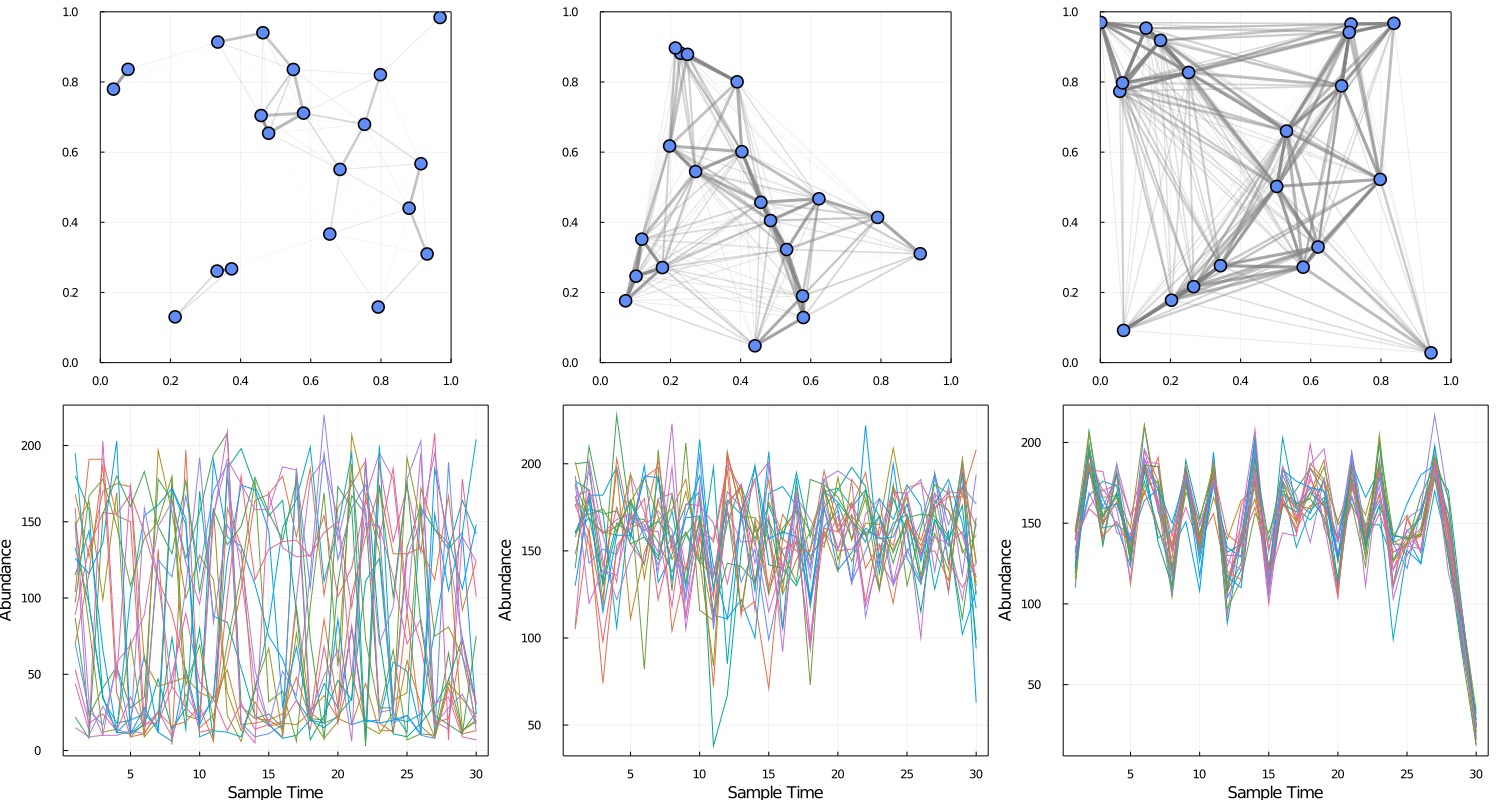
\includegraphics{./figures/synchrony_example.png}
\caption{TODO Caption}\label{fig:example}
}
\end{figure}

\hypertarget{methods}{%
\section{Methods}\label{methods}}

Here, we present a model of metapopulation dynamics on spatial graphs.
This model contains three parts: a model of landscape connectivity, a
model of local population dynamics, and a model of dispersal. We use
this model to simulate time-series of metapopulation abundances using
both diffusion and stochastic models of dispersal, and then measure the
synchrony of population dynamics between populations. By comparing the
synchrony created by stochastic dispersal and diffusion models, we show
there are two distinct regimes: a regime where diffusion well
approximates stochastic dispersal, and a regime where it does not.

\hypertarget{landscape-connectivity-model}{%
\subsection{Landscape connectivity
model}\label{landscape-connectivity-model}}

Spatial graphs have long been used to model a system of habitat patches
(nodes) connected by dispersal (edges, which combined form a landscape
(Urban \& Keitt 2001; Minor \& Urban 2008; Dale \& Fortin 2010).

// have to define connectivity

To describe how the edges of this spatial graph describe dispersal,

we model landscape connectivity as a combination of two different
factors: the probability than any individual migrates during its
lifetime, \(m\), and the conditional distribution over spatial nodes of
where an individual goes (\(j \in L\)), given both that it migrates
\(m\) and where it started (\(i \in L\)), which we call the dispersal
potential and denote

\[\Phi_{ij} =  P(i \to j | m)\]

The dispersal potential can be modeled several ways. In empirical
systems, the relative cost of movement from one point to another is
often estimated with resistance surfaces {[}spear\_use\_2010{]}. Here we
model the dispersal potential using isolation-by-distance (IBD), which
assumes the relative probability of dispersal from location \(i\) to
location \(j\) is inversely proportional to the distance between them,
\(d_{ij}\), and the strength of this IBD relationship, \(\alpha\), which
is treated as an intrinsic value of a species dispersal capacity. The
form of the IBD relationship (historically called the dispersal kernel)
we consider an exponential with decay-strength \(\alpha\) and a cutoff
value \(\epsilon\) (Hanski 1994; Grilli \emph{et al.} 2015).

\[f(d_{ij}, \alpha, \epsilon) =  \begin{cases} e^{-\alpha d_{ij}}
\quad\quad\quad &\text{if}\quad e^{-\alpha d_{ij}} > \epsilon \ \
\text{and } i \neq j \\   0 &\text{else} \end{cases}\]

Then, to construct a dispersal potential \(\Phi_{ij}\) with a kernel
\(f(d_{ij}, \alpha)\), we normalize:

\[\Phi_{ij} = \frac{f(d_{ij}, \alpha, \epsilon)}{\sum_k
f(d_{ik},\alpha, \epsilon)}\]

Note that the sum of each row of \(\Phi\), forms a probability
distribution, i.e.~\(\sum_j \Phi_{ij} = 1 \ \ \forall i\), meaning the
probability that an individual leaves its original population given that
it migrates is 1. In some cases, for a given location \(i\), the
dispersal kernel \(f(d_{ij}, \alpha, \epsilon)\) could be \(0\) for all
\(j\), in which case \(\Phi_{ii}\) is set to \(1\) to enforce this
condition. In all other cases, \(\Phi_{ii}=0\). Also note that if
\(\alpha=0\), the dispersal potential is a uniform distribution over
other locations. In Figure \ref{fig:mp}, we can see the same set of
points plotted spatial graphs plotted representing the same set of
populations across differing values of isolation-by-distance strength,
\(\alpha\).

\hypertarget{local-population-dynamics-model}{%
\subsection{Local population dynamics
model}\label{local-population-dynamics-model}}

We model local population dynamics using the Ricker Model. At each
timestep, the abundance \(N_i\) at location \(i\) is drawn as

\[N_i(t+1) \sim \text{Poisson}\bigg(N_i(t) \lambda R e^{- \chi
N_i(t)}\bigg)\]

where \(\chi\) represents the strength of mortality of surviving until
adulthood, \(R\) is the probability that an adult reproduces (\(0.9\)
for all results presented here), and where \(\lambda\) is the mean
number of offspring for each individual that reproduces---yielding three
total parameters: \(\theta = \{\lambda, R, \chi \}\). We consider the
simplest variation on the model, which only includes demographic
stochasticity, however it is straightforward to extend this to other
forms of stochasticity (\textbf{Melbourne2008ExtRis?}).

\hypertarget{dispersal-models}{%
\subsection{Dispersal Models}\label{dispersal-models}}

\hypertarget{stochastic-dispersal}{%
\subsubsection{Stochastic Dispersal}\label{stochastic-dispersal}}

To simulate stochastic dispersal, the number of migrants leaving a given
location is stochasticly drawn each timestep as
\(m_{i} \sim \text{Binomial}(N_i, m)\) for each location \(i\). For
every migrating individual we randomly draw where that individual goes
from the distribution of potential destinations \(\Phi^{(i)}\).

\hypertarget{diffusion}{%
\subsubsection{Diffusion}\label{diffusion}}

To simulate diffusion dispersal, we incorporate the local Ricker Model
into a reaction-diffusion model. If the probability that an individual
disperses before reproducing is \(m\), then we can define a diffusion
matrix \(D\) as

\[D_{ij} = \begin{cases} \Phi_{ij}m \quad\quad\quad &\ i \neq j \\ 1-m
& i=j \end{cases}\]

where \(D_{ij}\) is now the expected value an individual born in \(i\)
reproduces in \(j\). The dispersal dynamics of the diffusion model are
described by the mapping

\[N_i(t+1) = \sum_j D_{ji} N_j(t)\]

which can be combined into the local Ricker model from above as
reaction-diffusion model by computing diffusion before each round of
local dynamics.

\[N_i(t+1) \sim \text{Poisson}\bigg( \lambda R e^{-\chi \big(\sum_j
D_{ji} N_j(t)\big)} \cdot \sum_j D_{ji} N_j(t) \bigg)\]

\hypertarget{measuring-synchrony}{%
\subsection{Measuring Synchrony}\label{measuring-synchrony}}

In ecology and other fields, the crosscorrelation function, (CC), has
long been used as a measure of the synchrony between two time-series.
Here, with a metapopulation, we consider the mean crosscorrelation in
abundances between all pairs of populations, which we call
Pairwise-Crosscorrelation (\(\text{PCC}\)) and compute as

\[\text{PCC}=\frac{1}{(N_p-1)^2}\sum_{i \neq j} CC(\vec{N_i},\vec{N_j})\]

where \(\vec{N_i}\) is the time-series of abundances at population
\(i\).

\hypertarget{results}{%
\section{Results}\label{results}}

We first consider how synchrony, measured by \(\text{PCC}\), changes as
a function of the intrinsic dispersal probability \(m\). In figure
fig.~\ref{fig:migration_gradient}, we see how \(\text{PCC}\) changes in
response to \(m\) at varying levels of both landscape connectivity
\(\alpha\) and intrinsic growth rate \(\lambda\). We see that under some
combinations of \(\alpha\), \(\lambda\), and \(m\) both stochastic
dispersal (green) and diffusion (orange) produce similar levels of
synchrony, however at some parameter values diffusion artificially
creates more synchronous dynamics than stochastic dispersal.

\begin{figure}
\hypertarget{fig:migration_gradient}{%
\centering
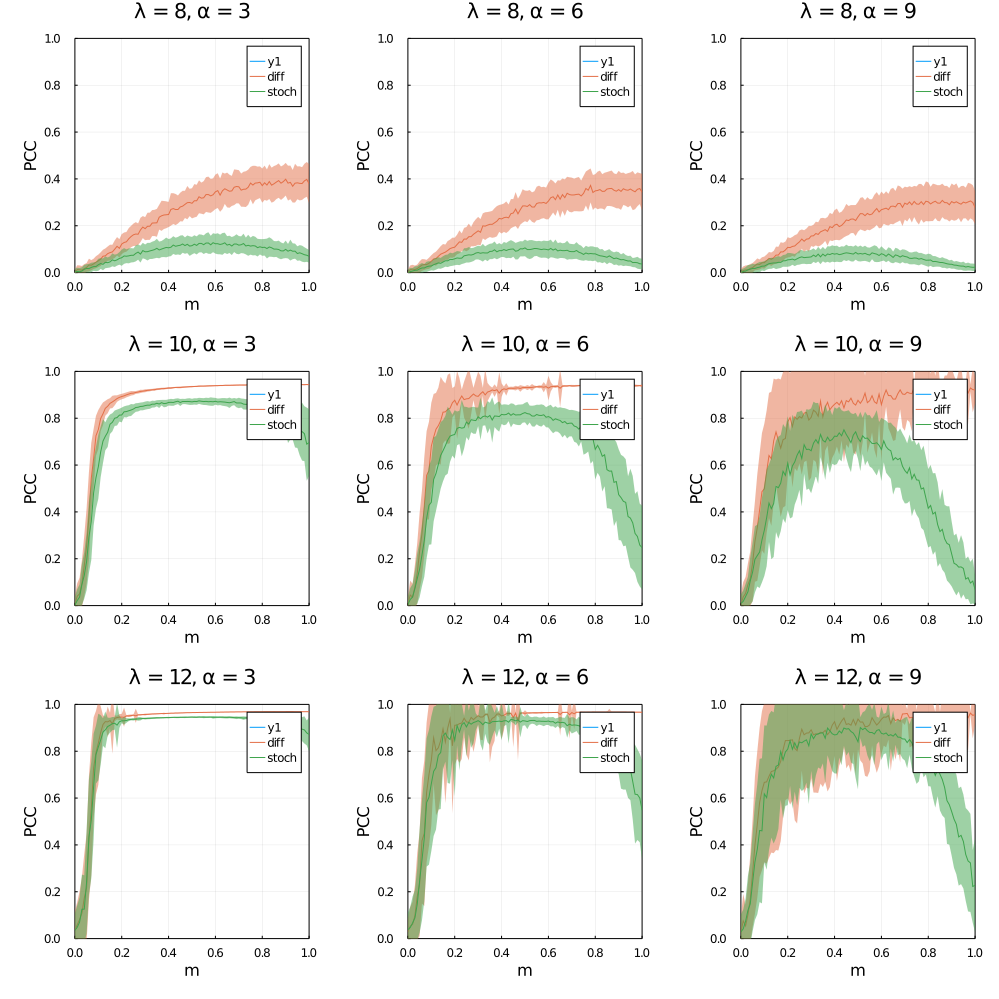
\includegraphics{./figures/migration_gradient_panels.png}
\caption{TODO Caption}\label{fig:migration_gradient}
}
\end{figure}

At low \(\lambda\), the diffusion model produces increasingly
synchronized population dynamics as migration increases; however, the
stochastic dispersal model produces effectively no synchrony regardless
of migration rate. As \(\lambda\) increases, we see two phenomena: 1)
the distribution of \(\text{PCC}\) for both diffusion and stochastic
model begin to move closer to one another, and 2) the shift from
non-synchronized to synchronized dynamics becomes more ``critical,''
meaning it rapidly jumps to near \(\text{PCC}=1.0\) as \(m\) increases.
As we increase \(\lambda\), the gap between the diffusion and stochastic
PCC distributions shrinks. As \(\alpha\), the modularity of the habitat
networks, increases, we see the difference in PCC between diffusion and
stochastic dispersal models shrink, but the amount of variance in this
estimate increases and we increase the modularity of the habitat network
(\(\alpha\)). In this case, the spatial configuration of habitat
patches, and how the dispersal structure of a randomly generated habitat
network changes with \(\alpha\), is driving greater variation in the
amount of synchrony observed at a given set of parameter values.

To better understand this, we consider ``mapping'' this difference in
the parameter space defined by varying levels of landscape connectivity
\(\alpha\) and intrinsic growth rate \(\lambda\) at ``snapshots'' of
various value of intrinsic dispersal rate \(m\)
(fig.~\ref{fig:lattice}). Dispersal rate is often treated as a property
intrinsic to a species.

\begin{figure}
\hypertarget{fig:lattice}{%
\centering
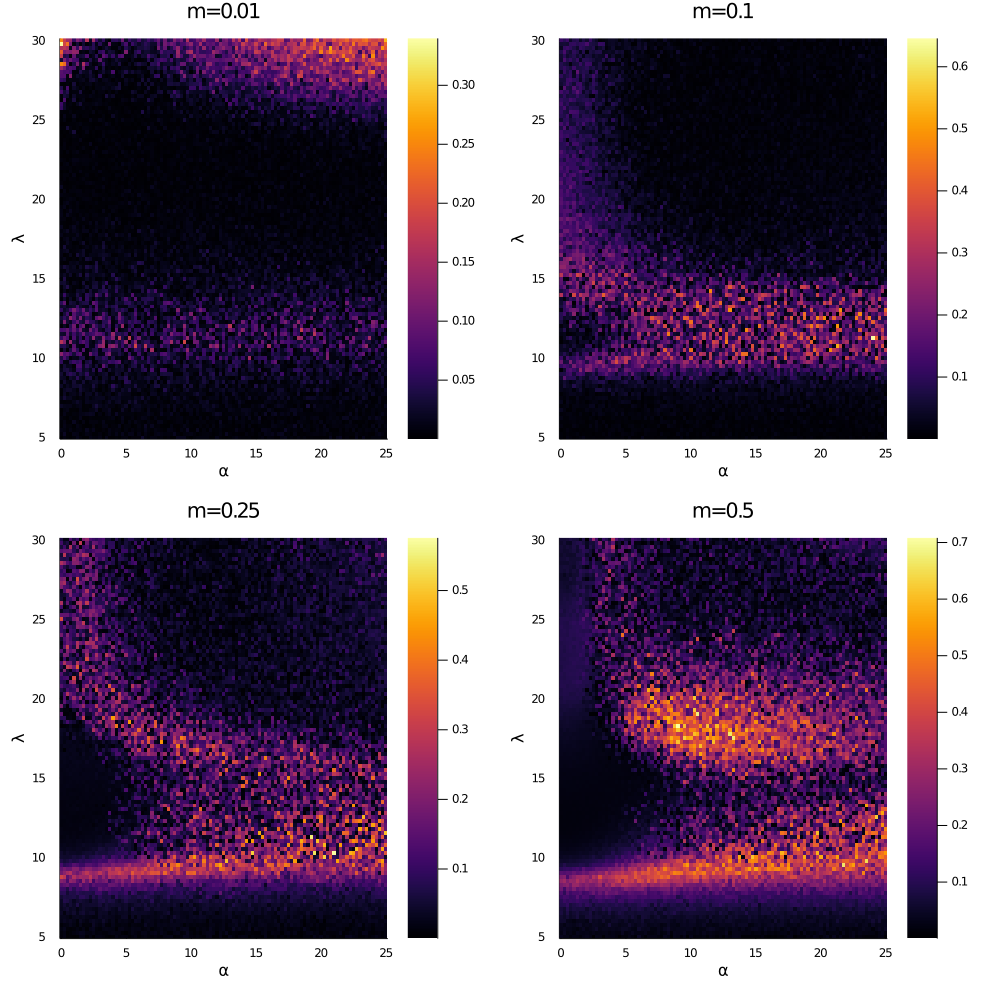
\includegraphics{./figures/connectivity_demography_lattice.png}
\caption{TODO Caption}\label{fig:lattice}
}
\end{figure}

Why is it that we see a response to \(\lambda\)? Consider what we know
about the Ricker model,By comparing the synchrony created by stochastic
dispersal and diffusion models, we show there are two distinct regimes:
a regime where diffusion well approximates stochastic dispersal, and a
regime where it does not.

higher \(\lambda\) without changing other parameters means the mean
population size increases. As the mean population size increases, the
size of the sampling distribution of dispersers at each timestep
increases, and we expect this distribution to converge to \(\Phi\) as
the number of migrants increases toward infinity.

We conclude by emphasizing the difference in simulation time between
these models, especially as the number of spatial locations increases.
This is compounded by stochastic dispersal's runtime is sensitive to the
intrinsic migration probability \(m\). At higher value of \(m\), more
dispersal events occur,

\begin{figure}
\hypertarget{fig:runtime}{%
\centering
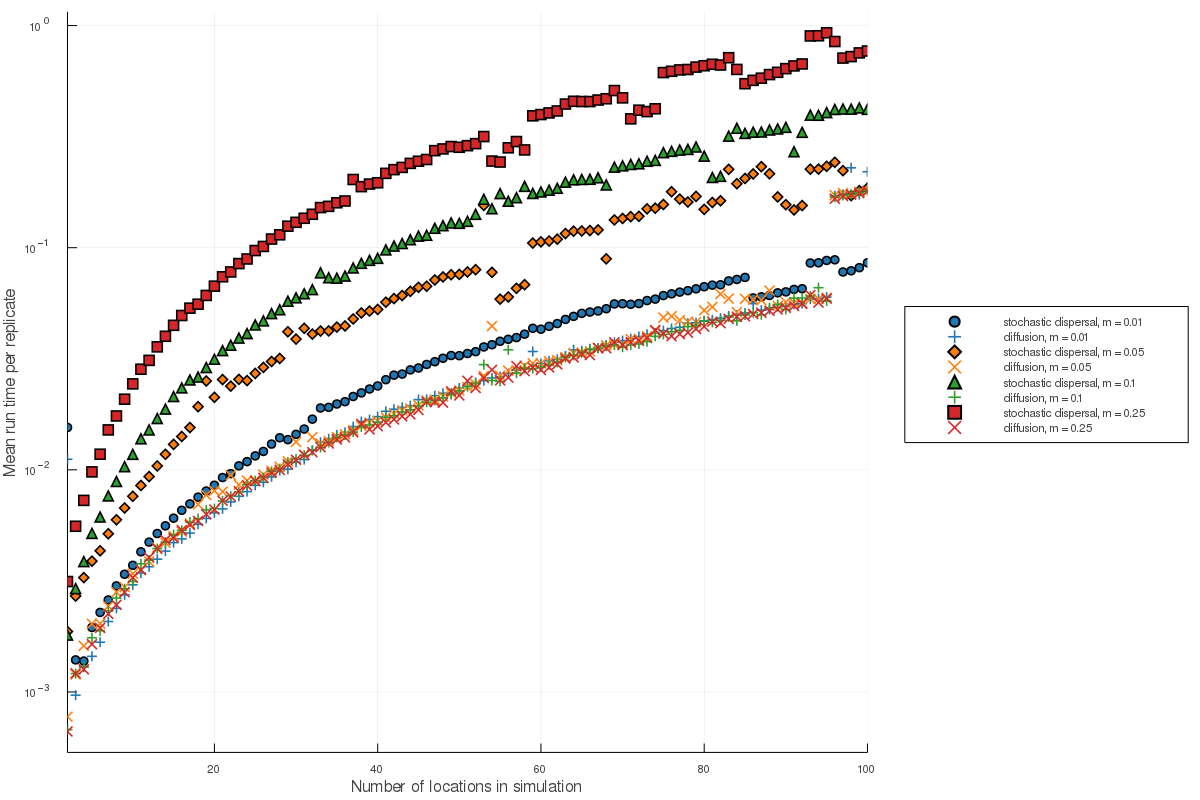
\includegraphics{./figures/runtime.png}
\caption{TODO Caption}\label{fig:runtime}
}
\end{figure}

\hypertarget{discussion}{%
\section{Discussion}\label{discussion}}

When developing models to understand and predict how landscape structure
effects ecological processes, diffusion can be a convenient abstraction
to speed up computation in some cases.

Here we show that diffusion can artificially synchronize dynamics across
space.

Spatial synchrony of population dynamics is generally of interest.
Dispersal induced synchrony can increase population stability, up until
a certain threshold where the dynamics become so highly synchronized
that they increase extinction risk (Abbott 2011).

The point goes beyond synchrony. The major point we intend to make here
is that if one is developing an ecological model that involves organisms
moving across space, it is imperative to test whether stochastic and
diffusion dispersal produce similar results. Diffusion can often be a
valuable abstraction that make computation faster. ``Understanding the
scope and proprer domain of each abstraction'' (Levins \& Lewontin 1987)
One way to view this is diffusion ignores temporal variation in
dispersal.

Another important consideration for this work is what is meant by a
``location'' within our model. Although we frame this in terms of
habitat patches, what an individual point in a spatial network
represents is a convenient abstract to represent the spatial dimension
of ecological processes. We argue the dispersal potential, by using
probabilistic framework to represent dispersal, is a way to describe
landscape structure at any scale.

\begin{itemize}
\tightlist
\item
  Spatial graph models as tool for modeling ecological processes across
  space and as generative models.
\item
  Emergent properties and the role of stochasticity
\end{itemize}

\hypertarget{acknowledgments}{%
\subsubsection{Acknowledgments}\label{acknowledgments}}

\hypertarget{references}{%
\section*{References}\label{references}}
\addcontentsline{toc}{section}{References}

\hypertarget{refs}{}
\begin{CSLReferences}{1}{0}
\leavevmode\hypertarget{ref-Abbott2011DisPar}{}%
Abbott, K.C. (2011). A dispersal-induced paradox: Synchrony and
stability in stochastic metapopulations. \emph{Ecology Letters}, 14,
1158--1169.

\leavevmode\hypertarget{ref-Albert2017AppNet}{}%
Albert, C.H., Rayfield, B., Dumitru, M. \& Gonzalez, A. (2017). Applying
network theory to prioritize multispecies habitat networks that are
robust to climate and land-use change. \emph{Conservation Biology}, 31,
1383--1396.

\leavevmode\hypertarget{ref-Dale2010GraSpa}{}%
Dale, M.R.T. \& Fortin, M.-J. (2010). From Graphs to Spatial Graphs.
\emph{Annual Review of Ecology, Evolution, and Systematics}, 41, 21--38.

\leavevmode\hypertarget{ref-Grilli2015MetPer}{}%
Grilli, J., Barabás, G. \& Allesina, S. (2015). Metapopulation
Persistence in Random Fragmented Landscapes. \emph{PLOS Computational
Biology}, 11, e1004251.

\leavevmode\hypertarget{ref-Hanski1994PraMod}{}%
Hanski, I. (1994). A Practical Model of Metapopulation Dynamics.
\emph{The Journal of Animal Ecology}, 63, 151.

\leavevmode\hypertarget{ref-Hastings1978GloSta}{}%
Hastings, A. (1978). Global stability in Lotka-Volterra systems with
diffusion. \emph{Journal of Mathematical Biology}, 6, 163--168.

\leavevmode\hypertarget{ref-Levins1987DiaBio}{}%
Levins, R. \& Lewontin, R.C. (1987). \emph{The Dialectical Biologist}.
Harvard University Press, Cambridge, Mass.

\leavevmode\hypertarget{ref-Minor2008GraFra}{}%
Minor, E.S. \& Urban, D.L. (2008). A Graph-Theory Framework for
Evaluating Landscape Connectivity and Conservation Planning.
\emph{Conservation Biology}, 22, 297--307.

\leavevmode\hypertarget{ref-Resasco2019MetDec}{}%
Resasco, J. (2019). Meta-analysis on a Decade of Testing Corridor
Efficacy: What New Have we Learned? \emph{Current Landscape Ecology
Reports}, 4, 61--69.

\leavevmode\hypertarget{ref-Urban2001LanCon}{}%
Urban, D. \& Keitt, T. (2001). Landscape Connectivity: A Graph-Theoretic
Perspective. \emph{Ecology}, 82, 1205--1218.

\end{CSLReferences}

\end{document}
